\documentclass[11pt]{article}
%Gummi|065|=)
\usepackage[english]{babel}
\usepackage{graphicx}
\title{\textbf{Welcome to Gummi 0.6.5}}
\author{Alexander van der Mey\\
		Wei-Ning Huang\\
		Dion Timmermann}
\date{}
\begin{document}


\section{Future Research}
A potential route to further the inferences in this paper would be be investigate and perform variable selection based on the correlations between the predictors within the data. This is discussed very briefly below.

We can form the model matrix of the data providing we have converted the necessary predictors into factors. From this model matrix which contains only binary indicator variables we can form the correlation matrix. 

\begin{figure}[h!]
  \caption{Factors' correlation matrix.}
  \centering
    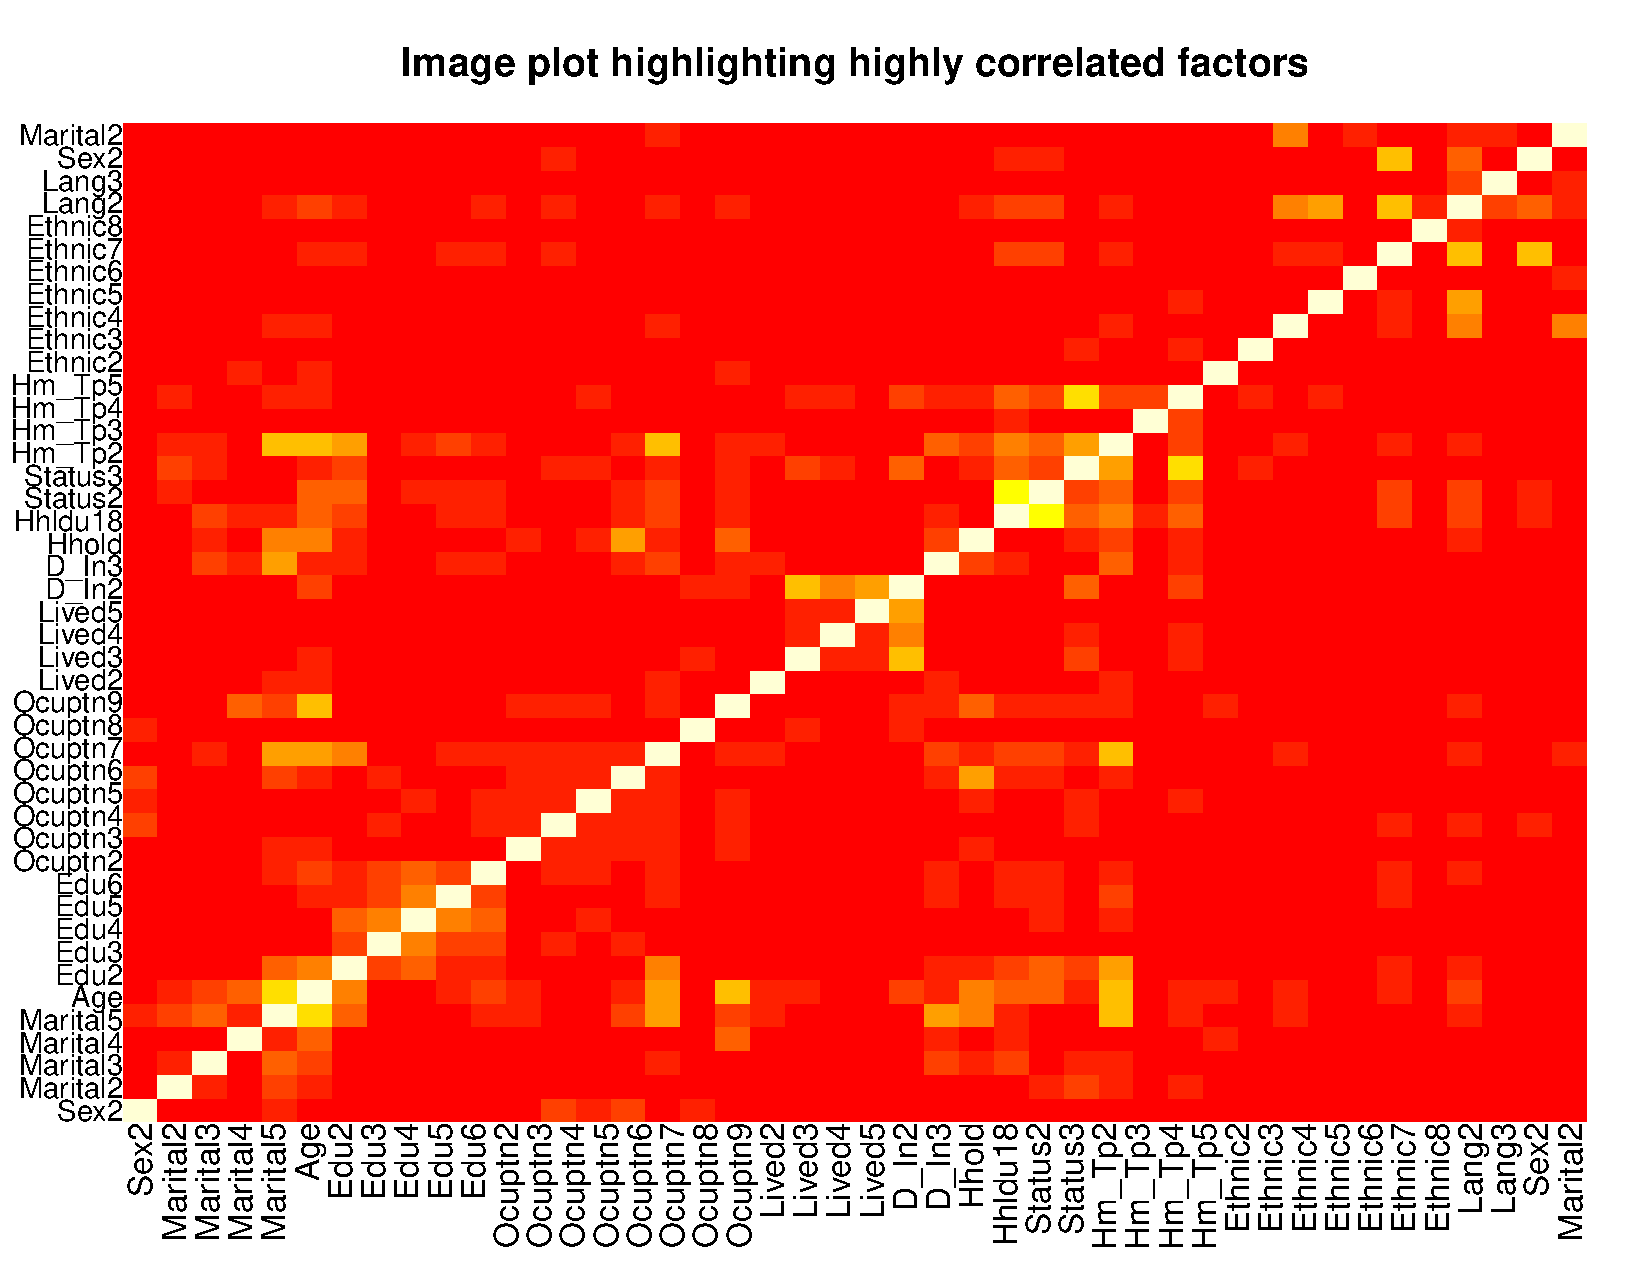
\includegraphics[width=1.0\textwidth]{HandlingMissingDataAndFutureReseachPlots/CorrImageNoThresh.pdf}
\end{figure}

This 42x42 matrix contains a lot of information pertaining to the marginal relations of every pair of levels of predictors in the model.

We can add threshold to the matrix to only only highlight those pairs we deem to have a significant correlation, say an absolute value greater than 0.5. With this being a symmetric matrix it is sufficient to only inspect the those correlation which lie above the main diagonal. 

\begin{figure}[h!]
  \caption{Factors' correlation matrix with threshold.}
  \centering
    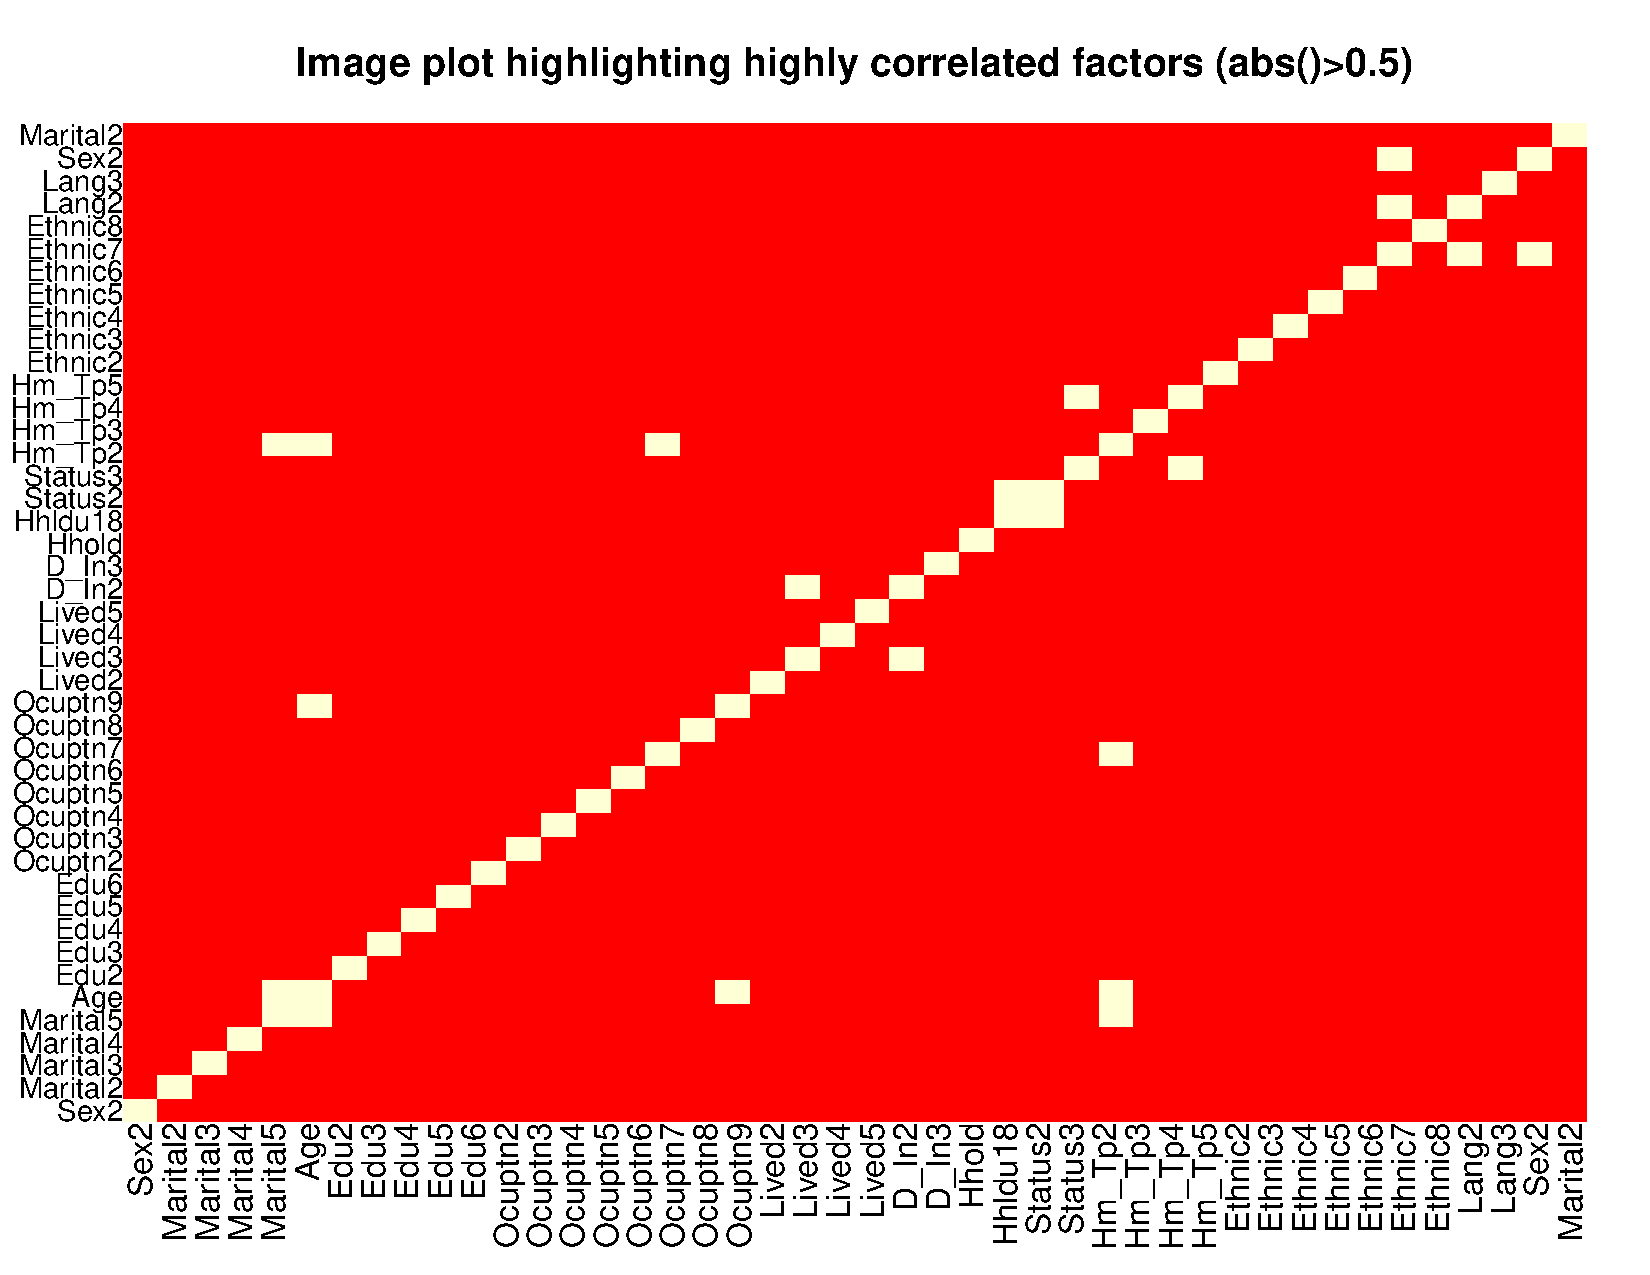
\includegraphics[width=1.0\textwidth]{HandlingMissingDataAndFutureReseachPlots/CorrImageWithThresh.pdf}
\end{figure}

From the plot below we see that there are ten such pairs of predictors.

\end{document}